\section{Data, stripping, and simulation}

The data collected by the \lhcb detector used in this thesis totals $3\invfb$; where $1\invfb$ was
collected in the year 2011 with a centre-of-mass energy of $7\tev$, and $2\invfb$ at $8\tev$ was
collected in 2012.
In total, the data collected in 2011 and 2012 is known as Run-1 data.

%\subsection{Stripping}
Even the much reduced \hlttwo output rate of $5\khz$ is a vast amount of data for an
analyst to sift through in a timely manner.
To improve the speed to access data, additional selections are applied to the dataset biannually
which further categorise each event.
This is known as stripping.
Stripped datasets are the only ones accessible to analysts, which makes the process of retrieving
data of interest fast.
Stripping selections in this thesis vary, and will be described when appropriate.


%\deleted{
%%\section{Simulation}
%Reliable analysis of real data would not be possible without selections of simulated events.
%%Simulation of events is a vital part of analyses at \lhcb, it allows collaborator's access to pure
%These allows collaborator's access to pure samples of specific, requested decays to aid their
%research.
%This can be for the evaluation of efficiencies, understanding effects in data, or making analysis
%decisions without compromising blinded data.
%These events are generated in two independent phases: generation and simulation.
%Proton-proton collisions are generated using \pythia
%with a specific \lhcb configuration,
%and subsequent hadronic decays are handled by the \evtgen package.
%The simulation phase is designed to mimic the \lhcb detector's response to particles, this is done
%with \geant as described in
%Ref.
%}
%%Simulated events after the hadronization stage and before detector modelling are known as
%%\emph{generator level} simulation.



\added{
Simulated events are used in \lhcb analyses primarily for the purposes of optimising selections and
determining efficiencies.
Other important uses include the modelling of kinematic distributions and understanding various
sources of background.
The \lhcb collaboration produces simulated events in a pipeline consisting of multiple stages.
%Simulations produced by the \lhcb collaboration begin
%by modelling the $pp$ collisions, followed by
%the subsequent decays, and ending with the detector's response to the final state particles.
Proton-proton collisions are generated using \pythia~\cite{Sjostrand:2006za,*Sjostrand:2007gs} with
a configuration specific to \lhcb~\cite{LHCb-PROC-2010-056}, giving details of: the size of the
luminous region; the number of interactions per bunch crossing; and spill-over events from
neighbouring proton bunches.
Heavy flavour particles are produced by a hadronization process in \pythia.
Subsequent decays are modelled with
\evtgen~\cite{Lange:2001uf}, which is a package created specifically for modelling the decays of
heavy flavour particles.
The composition of decays in each sample of simulated events is requested at this level, and
\evtgen forces one of the heavy flavour quarks to decay accordingly, other heavy quarks proceed to
decay via a random decay chain.
Selection cuts are applied throughout and if the required quark of heavy
flavour is produced in the backward direction the $z$-coordinates are flipped, this is to save time
at later stages.
At this stage,the simulation is known as \emph{generator level}, which can be useful for
determining distributions before the detector interactions have been accounted for.
Final state radiation is modelled using \photos~\cite{Golonka:2005pn}.
The interactions of each particle with the \lhcb detector is modelled using
\geant~\cite{Allison:2006ve,*Agostinelli:2002hh} as described in Ref.~\cite{LHCb-PROC-2011-006}.
Trigger decisions are applied to the simulation, however events which do not pass various triggers
are not discarded, and instead are stored.
After the simulation is complete, events are treated identically to the collected data; being
processed by the same stripping selections.
}


\added{
Considering the importance of simulated events it is important for them to be trusted.
To this end each analysis must ensure that the simulation used describes the data to a good degree,
sometimes it is necessary for weights to be applied to correct for small differences.
This is particularly true for \pid variables, which are known to be poorly modelled by the
simulation.
That being said, the simulated events are seen to reproduce data distributions very accurately.
Figure~\ref{fig:data:ipres} shows the \gls{IP} resolution as a function of the inverse \pt of a
track, the performance is roughly linear in this variable.
The \velo achieves \gls{IP} resolutions of less than $25\mum$ for particles with $\pt>1\gev$, and
}
the agreement between data and simulation is seen to be excellent~\cite{LHCb-DP-2014-001}.


\begin{figure}
  \begin{center}
    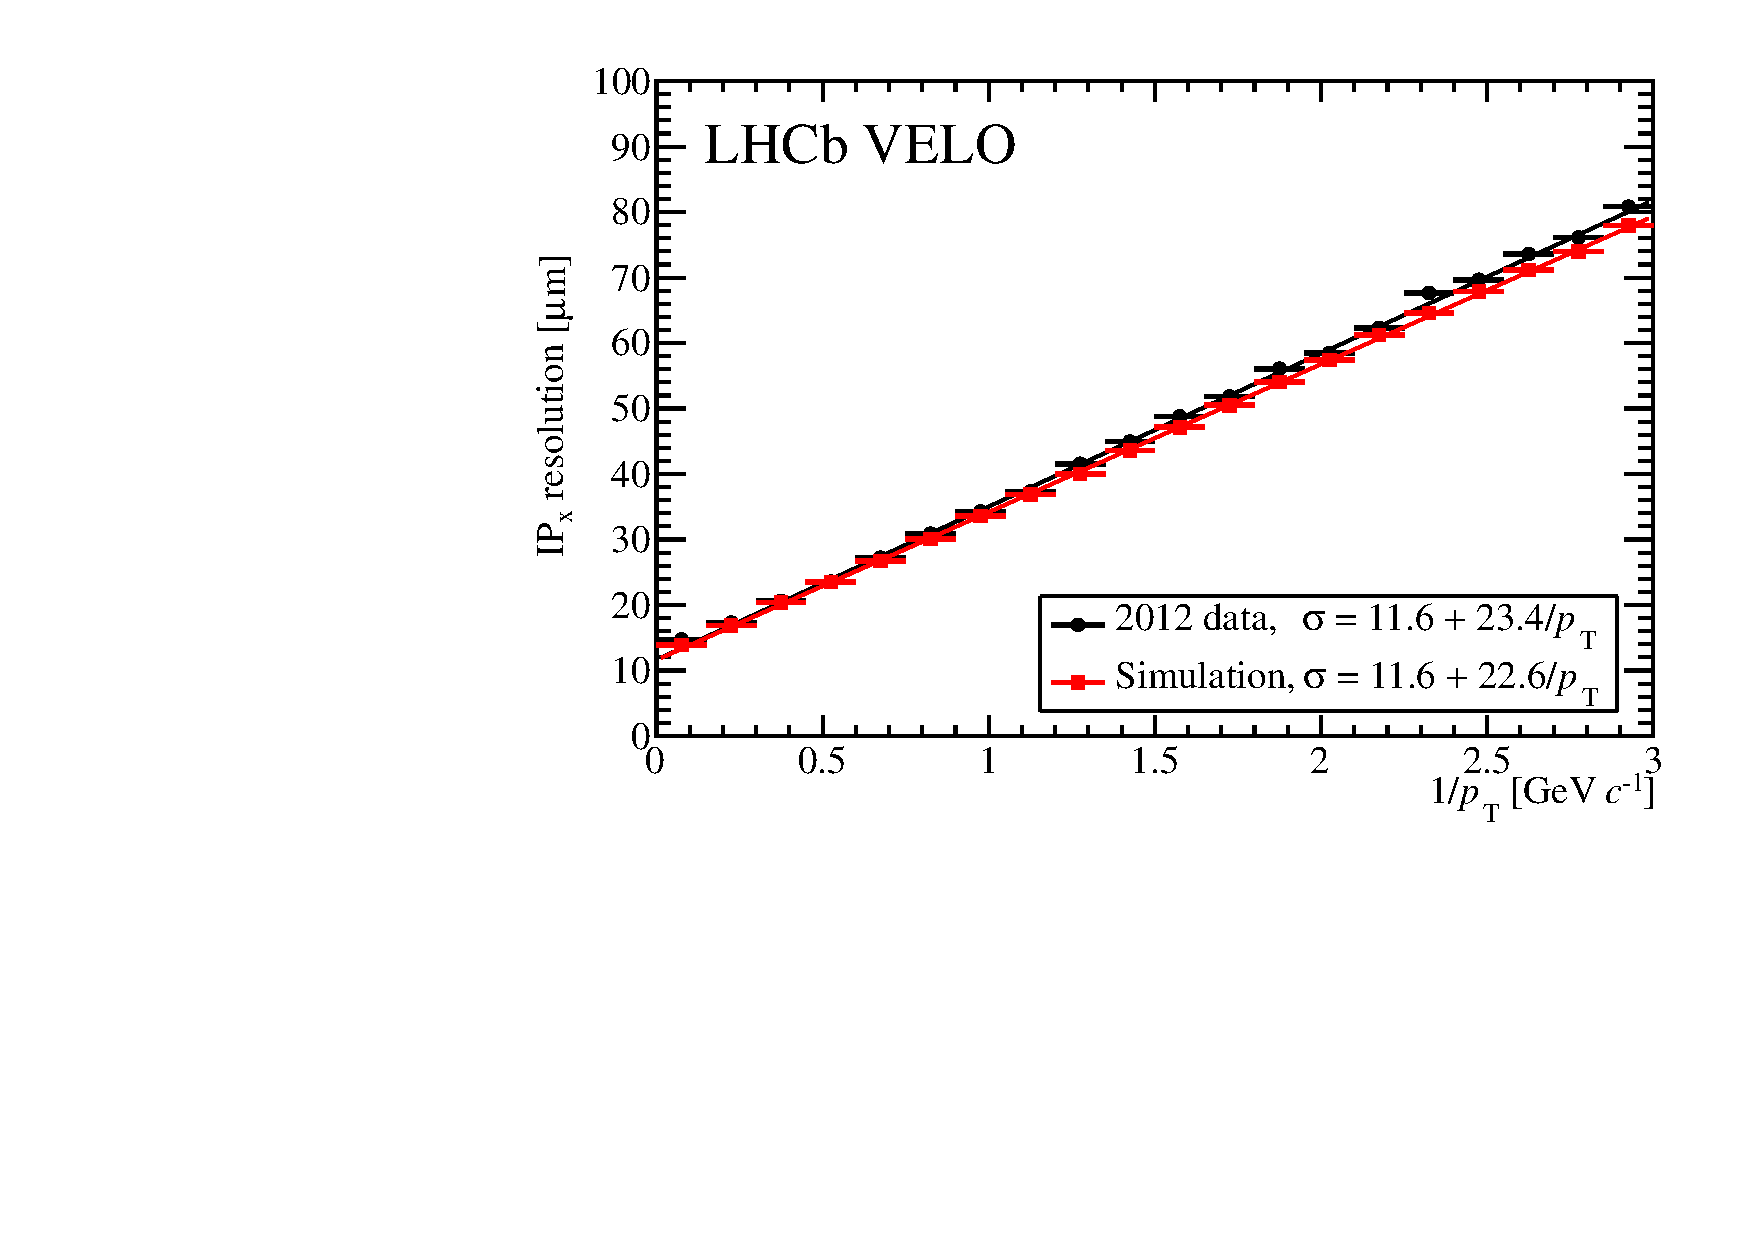
\includegraphics[width=0.48\textwidth]{IPXRes_invp}
    \caption[Impact parameter resolution as a function of inverse transverse momentum comparing
      data and
    simulation]{
      Impact parameter resolution as a function of a track's inverse transverse momentum comparing
      (black)
      data taken in 2012 which is also shown in Fig.~\protect\ref{fig:velo:ipres} and (red)
      simulation.  Excellent agreement is seen, particularly for high momenta tracks,
      $\pt>1\gev$~\protect\cite{LHCb-DP-2014-001}.
    }
    \label{fig:data:ipres}
  \end{center}
\end{figure}




%%%%%%%%%%%%%%%%%%%%%%%%%%%%%%%%%%%%%%%%%%%%%%%%%%%%%%%%%%%%%%%%%%%%%%%%%%%%%%%%

%The high output rate of the \lhcb trigger means that there is a huge amount of data to be made
%accessible to collaborators, too much to be convenient, in fact.
%Because of \lhcb's wide physics program it is possible to run further collaboration wide selection
%twice a year to reduce the dataset by approximately a factor of ten.
%Within each of these data-subsets further stripping flags are applied which further increase the
%speed which a dataset can be processed.
%The stripping lines used in this thesis are the Dimuon line and the
